\documentclass[12pt]{article}
\usepackage[utf8]{inputenc}
\usepackage[a4paper,margin=1in]{geometry}
\usepackage{amsmath} 
\usepackage{amssymb}
\usepackage{graphicx}
\usepackage{float}
\usepackage{tabularx} 
\usepackage{caption}
\usepackage{subcaption}
\usepackage{array}
\usepackage{listings}
\usepackage{pythonhighlight}



\title{
    Department Of Aerospace Engineering,\\
    Indian Institute Of Technology Madras
    \begin{figure}[H]
        \centering
        
\includegraphics[width=8cm]{iitmlogo.png}
    \end{figure}
    \begin{center}
        \textbf{\\AS2101 : Introduction to Aerospace Engineering\\}
        Report 7\\
    \end{center}
}
\author{
    Pranit Zope\\AE20B046
}
\date{\today}

\begin{document}
\pagenumbering{gobble}
\maketitle
\newpage
\pagenumbering{arabic}
\tableofcontents 
\listoffigures

\newpage


\section{Aim}
To Find the Integral
\begin{equation*}
    \int_{-1}^1 e^{-x}sin^2(4x)
\end{equation*} using Trapezoidal and Gaussian Quadrature and comparing the efficiency of both the techniques.

\section{Theory}
\subsection{Fundamental Rule of Gaussian Quadrature}
This is used to find the exact values of definite integrals of polynomials (degree = 2n-1, where n is the number of nodes solved.)
\begin{equation}
    \int^1_{-1} f(x)dx = \sum^n_{i=0}f(x_i) \cdot w_i  
\end{equation}
Here, $w$ is called the weighted sum.

\subsection{Gauss-Legendre Quadrature}
To find the weighted sum $(w)$, we need a set of orthogonal polynomials called the \textbf{Legendre Polynomials} which are given by Rodrigue's formula, which states
\begin{equation*}
    P_n(x) = \frac{1}{2^n n!} \cdot \frac{d^n}{dx^n} (x^2-1)^n
\end{equation*}
The roots of $P_n(x)$ are the nodes used. After this, we calculate th weighted sum byt the formula :
\begin{equation*}
    w_i(x) = \frac{2}{(1-x_i^2)[(P_n(x_i)]^2}
\end{equation*}

\subsection{Trapeziodal Method of Integration}
We divide the area under curve into several trapezoids and sum up the area to ultimately find the value of definite integral.
\begin{figure}[H]
    \centering
    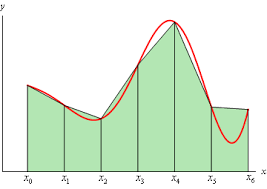
\includegraphics[width=8cm]{trap.png}
    \caption{Trapezoidal Method of Integration}
\end{figure}
\begin{equation*}
    I = \sum^n_{i=0} \frac{(x_{i+1}-x_{i})(f(x_i) + f(x_{i+1}))}{2}
\end{equation*}

\subsection*{Legendre Polynomials}
\begin{figure}[H]
    \centering
    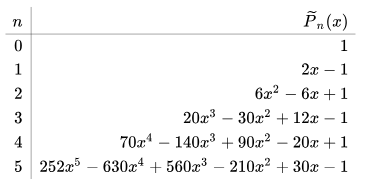
\includegraphics[width=10cm]{leg.png}
    \caption{First 5 Legendre Polynomials}
\end{figure}

\subsection*{Nodes and weights}
\begin{figure}[H]
    \centering
    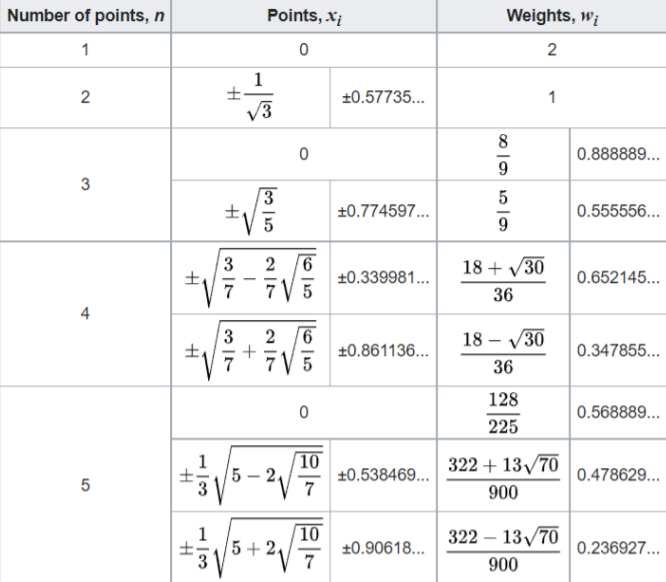
\includegraphics[width=10cm]{weg.png}
    \caption{Nodes and Weight Sums of first 5 n}
\end{figure}

\subsection{Change of Limits}
As we can see in the Fundamental rule of Gaussian Quadrature, the limits give us integrals inly from -1 to 1.\\
Thus, in order to change the limits from (-1 to 1) to (a to b), we use $x=\frac{b-a}{2} u+\frac{b+a}{2}$ such that we can get the required integral by putting u from -1 to 1.
\begin{equation*}
    \int_{a}^{b} f(x) d x=\int_{-1}^{1} f\left(\frac{b-a}{2} u+\frac{b+a}{2}\right) d u
\end{equation*}



\section{First 5 Legendre Polynomials - Graphical Representation}
\begin{figure}[H]
    \centering
    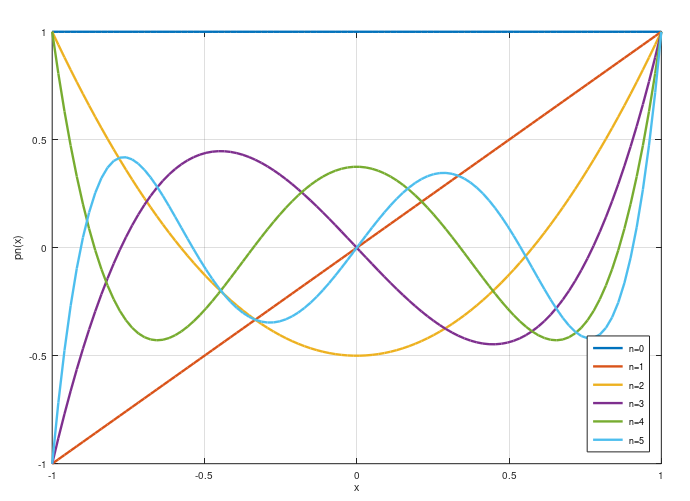
\includegraphics[width=13cm]{5leg.png}
    \caption{Graphical Representation of first 5 Legendre polynomials}
\end{figure}

\section{Manual Integration}
We will find the value by manual integration first, and then later tally with the results of the Trapezoidal and gaussian Method.
\begin{equation*}
    I=\int_{-1}^{1} e^{-x} \sin ^{2}(4 x) d x
\end{equation*}
As we know, $f(x) \equiv f(a+b-x)$;
\begin{equation*}
    I=\int_{-1}^{1} e^{x} \sin ^{2}(4 x) d x
\end{equation*}
Solving this, we get 
\begin{equation*}
    I = [-\frac{e^{x}}{130}[8 \sin (8 x)+\cos (8 x)-65]^1_{-1}
\end{equation*}
Which on putting limits gives us \\
$I = 0.9899352767719962$

\section{Results using Trapezoidal and Gaussian Methods}
\subsection{Gaussian Method}
\begin{python}
>> gaussian(10)
ans = 0.989935015655239

>> gaussian(30)
ans = 0.989935276771999

>> gaussian(50)
ans = 0.989935276771994

\end{python}
\textit{*Code attached in appendix}

\subsection{Trapezoidal Method}
\begin{python}
>> trapezoidal(10)
ans = 1.036961178946498

>> trapezoidal(30)
ans = 0.994978738845161

>> trapezoidal(50)
ans = 0.991745973094080

\end{python}
\textit{*Code attached in appendix}

\section{Errors(log(error) vs N : Graphical Analysis}
\subsection{Gaussian Method}
\begin{figure}[H]
    \centering
    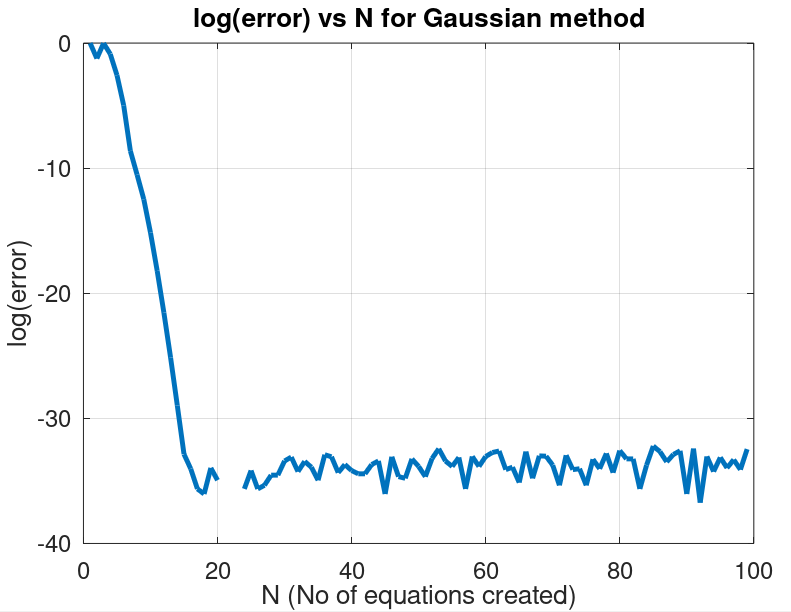
\includegraphics[width=10cm]{errg.png}
    \caption{log(error) vs N graph for Gaussian Method}
\end{figure}

\subsection{Trapezoidal Method}
\begin{figure}[H]
    \centering
    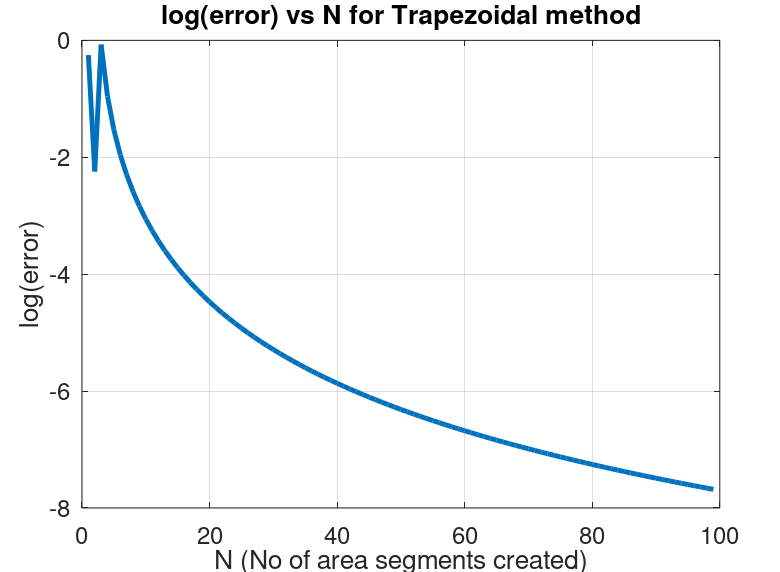
\includegraphics[width=10cm]{errt.png}
    \caption{log(error) vs N graph for Trapezoidal Method}
\end{figure}

\newpage
\appendix
\addcontentsline{toc}{section}{Appendix}

\section{.m code for Gaussian Method}
\begin{python}
# Pranit Zope
# AE20B046
# Task 06

function retval = gaussian (n)
format long
x=zeros(99);
w=zeros(100);
for i=1:99
file_name=int2str(i);
a=strcat(file_name,"roots.txt");
b=strcat(file_name,"weights.txt");
temp_1=importdata(a);
temp_2=importdata(b);
  for j=1:size(temp_1)(1,2)
    x(i,j)=temp_1(1,j);
  endfor
  for j=1:size(temp_2)(1,2)
      w(i,j)=temp_2(1,j); 
endfor
endfor
retval=0;
for k=1:99
  retval+=w(n,k)*f(x(n,k));
endfor
endfunction

\end{python}

\section{.m code for Trapezoidal Method}
\begin{python}
# Pranit Zope
# AE20B046
# Task 06

function retval = trapezoidal(n)
format long

x=linspace(-1,1,n+1);
retval=0;
for i=1:n
  retval+=0.50*(x(i+1)-x(i))*(f(x(i))+f(x(i+1)));
endfor
endfunction
\end{python}

\section{.m code for error analysis}
\subsection{Gaussian Method}
\begin{python}
# Pranit Zope
# AE20B046
# Task 06


format long;
x=1:99;
y1=[];
for i=1:99
  y1=[y1,log(error(gaussian(i)))];
endfor
gaussian(21)
plot(x,y1,"-",'linewidth',2.5)
grid on
title('log(error) vs N for Gaussian method')
xlabel('N (No of equations created)')
ylabel('log(error)')
set(gca,'fontsize',24)

\end{python}

\subsection{Trapezoidal Method}
\begin{python}

# Pranit Zope
# AE20B046
# Task 06

format long
x=1:99
y1=[]
for i=1:99
  y1=[y1,log(error(trapezoidal(i)))]
endfor
trapezoidal(99)
plot(x,y1,"-",'linewidth',2.5)
grid on
title('log(error) vs N for Trapezoidal method')
xlabel('N (No of area segments created)')
ylabel('log(error)')
set(gca,'fontsize',24)

\end{python}
\end{document}